\documentclass[german]{report}
\usepackage[ngerman]{babel}
\usepackage[ansinew]{inputenc}
\usepackage{graphicx}
\usepackage{here}
\usepackage{pdfpages}
\usepackage{url}
\usepackage{amssymb,amsmath}
\usepackage{listings}
\usepackage{multirow}
\usepackage{fancyhdr}
\usepackage{lmodern}

\usepackage{color}
\usepackage{xcolor}
\usepackage{listings}

%\usepackage{caption}
%\DeclareCaptionFont{white}{\color{white}}
%\DeclareCaptionFormat{listing}{\colorbox{gray}{\parbox{\textwidth}{#1#2#3}}}
%\captionsetup[lstlisting]{format=listing,labelfont=white,textfont=white}



  \RequirePackage{draftwatermark}
  \SetWatermarkText{DRAFT}

\begin{document}

\pagestyle{fancy}
\lhead{\color{red}\textbf{DRAFT}}
\chead{- Knowledge Based Systems - }
\rhead{\includegraphics*[width=2.0cm]{abbildungen/dhbwlogo.png}}

\cfoot{Christoph Schabert, Stephan Alaniz, Jan Brodhacker (TINF11-AI\/BC) \\DHBW Mannheim}
\lfoot{\color{red}\textbf{DRAFT}}
\rfoot{\thepage}
\fancyhfoffset{\marginparsep}
\renewcommand{\footrulewidth}{1.0pt}
\renewcommand{\headrulewidth}{1.0pt}
\renewcommand{\headheight}{30pt}
\pagenumbering{arabic}





\begin{titlepage}

\begin{flushright}
    \includegraphics*[width=4.0cm]{abbildungen/dhbwlogo} \\ 
\end{flushright}
\begin{center}
\vspace{1.5cm}
\Huge{ \textsf{Knowledge Based Systems}} \\
	Yavalath\\
    \vspace{4cm}
 \normalsize{
    \begin{tabular}{ll}
    	Names: & {Schabert Christoph  Alaniz Stephan  Brodhacker Jan} \\
    	Course: & {TINF-AI11/BC}	\\
    	Lecturer: &  HR. Dr. Dr. Dr. Dr. Vossen\\
    	working period: & 09.09.2013 to XX.XX.2014
    \end{tabular}\\
    }
\end{center}

\end{titlepage}

\newpage
\section*{Statutory declaration}\thispagestyle{empty}
I herewith declare that I have completed the present thesis independently making use only of the specified literature and aids. Sentences or parts of sentences quoted literally are marked as quotations; identification of other references with regard to the statement and scope of the work is quoted. The thesis in this form or in any other form has not been submitted to an examination body and has not been published.\\
\\
Stephan Alaniz:\\
Heidelberg, the \_\_.\_\_.2013 \hspace{2.5cm} .............................. \\
\hspace*{6.5cm} (signature)\\
\\
Christoph Schabert:\\
Heidelberg, the \_\_.\_\_.2013 \hspace{2.5cm} .............................. \\
\hspace*{6.5cm} (signature)\\
\\
Jan Brodhacker:\\
Heidelberg, the \_\_.\_\_.2013 \hspace{2.5cm} .............................. \\
\hspace*{6.5cm} (signature)\\

\newpage
\setcounter{page}{1}



\tableofcontents

\listoffigures

\renewcommand{\lstlistlistingname}{Listing of Sourcode}
\renewcommand{\lstlistingname}{Sourcode}
\lstlistoflistings

\bibliographystyle{plain}
\bibliography{Quellen}

\newpage

\chapter{Intruduction}
\label{sec:chapter1}
\section{Goal and Motivation}
The goal of this project is to implement a game called Yavalath. And to develop
two different Artificial Intelligences, which are able to play the game and win
against nearly every human player.

\section{Technical Notes}
The implementation of the game and the ai-players with a fully functional
graphical user interface is availible on GitHub und the the following url:
\begin{quotation}
    https://github.com/belafarinrod91/KBSYavalath (hep: 25.10.2013)
\end{quotation}
This project is under no license or otherwise protected, feel free to clone the
Git repositry and compile it yourself.


This publication was written in \LaTeX an compiled with MikeTex.

\chapter{The Game - Yavalath}
\label{sec:chapter2}
In this chapter the history of Yavalath, and the game is explained.
% #TODO: tech more!!!
\section{History}
Yavalath is the most successgul game evolved by LUDI in 2007 and published in 2009 by Nestorgames (Spain). LUDI is a game-generating computer program 
that implements an algorithm for generating new games. This LUDI software system not only defines the scope and rules of the game, it also interpets 
the game and coordinates testplays to measures the game quality.
LUDI was developed by Cameron Browne as part of his PhD in AI and game design,
also was he awarded with the Dean's Award for Outstanding Thesis
\cite{EvolutionGameDesign}. \\

In 2011 Yavalath was ranked onto place 99 from the BoardGameGeek
community\footnote{\url{www.boardgamegeek.com}} out of 4300 abstract games ever invented.
It was also rated onto place 8 out of 200 abstract games invented in 2007. \\

Yavalath won 2012 the Humies Award for Human-Competitive Result Produced by Genetic and Evolutionarty Computation

\section{Categorisation}
Yavalath is a mixture of connect and patter building game. The BoardGameGeek
community categorised Yavalath as a abstract game because it was the first
computer-generated game with such a huge success.

Also Yavalath inspired a new game categorie thats called:
\begin{quote}
	winning with a line of N and losing with a line of N-1.
\end{quote}

The name Yavalath was randomly created by a Markovian algorithm.

\section{The Rules}
The Rules for Yavalath are pretty simple, what makes it easy to learn. But its
still novel so that the game is still intressting. 
One of the reasons why the game became so successfull is that Yavalath achieves
a good balance between simplysiti and a kind of innovation.

Yavalath is for two or three players and the average playingtime per game is 10 minutes\footnote{this was voted by the BoardGameGeek comunity, source:\url{http://boardgamegeek.com/boardgame/33767/yavalath}}.

The board is a hexagon with 5 spaces on every side, that is initally empty.
With that specifications there are 61 free cells in total, as to see in Illustration \ref{fig:yav_board}.

\begin{figure}[ht]
\centering
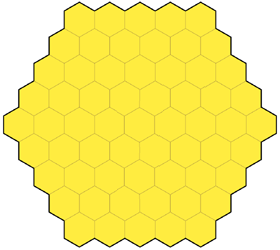
\includegraphics[width=0.95\textwidth]{Abbildungen/yav_emptyBoard.png}
\caption[The Yavalath game board, Source:\cite{yvalathHP}]{The Yavalath game board}
\label{fig:yav_board}
\end{figure}


Every turn a players place a pieces of their colour onto the board. 

This goes on untill:
\begin{itemize}
	\item on player have won
	\item all but one players have lost
	\item all cells are filled and it is a draw
\end{itemize}

As Soon as a Player formes a line of three pices in a row the player looses.

A player can win with two different methods:
\begin{enumerate}
	\item one players manage to make a line of four or more pices of his color (In illustartion  \ref{fig:yav_4inarow} the white player won).
	\item one player forece another player to form a line of three pices what is called a forced move. (In illustartion  \ref{fig:yav_forceMove} the black player is forced to move to prevent the white player from winning. in).
\end{enumerate}

\begin{figure}[ht]
\centering
\includegraphics[width=0.95\textwidth]{Abbildungen/yav_4inarow.png}
\caption[Four in a row wining, Source:\cite{yvalathHP}]{Four in a row wining}
\label{fig:yav_4inarow}
\end{figure}


\begin{figure}[ht]
\centering
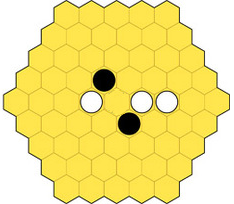
\includegraphics[width=0.95\textwidth]{Abbildungen/yav_forceMove.png}
\caption[Forced move winning, Source:\cite{yvalathHP}]{Forced move winning}
\label{fig:yav_forceMove}
\end{figure}


This leads to a so called Rule Tension, in this case four is a row is good but three in a row is bad. This means the Player cant just extend lines and must think about the pros and cons of every move he makes.\cite{yvalath}

\section{Tactics and Strategy}
Cameron Browne himsself defined some taktics and strategies and described them in his publication. He started to describes a number of chooices for the first move and a number of patterns that have a good chance of winning.


The first move is crucial for the folowing tactics and for the chance to win.
In Illustration \ref{fig:yav_winChance} is shown a Yavalath board with the win chance for the first move, the bigger the bouble the bigger the win chance. As its good visable that a centerd first move has the biggest win chance.\cite{yvalathHP}


\begin{figure}[ht]
\centering
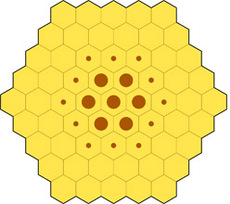
\includegraphics[width=0.95\textwidth]{Abbildungen/yav_winChance.png}
\caption[The win chance for the first Move, Source:\cite{yvalathHP}]{The win chance for the first Move}
\label{fig:yav_winChance}
\end{figure}


An other good chooice for a first move is to start with a pattern. The Triangle starting pattern is an excelent example for a first move pattern (the Triangle starting pattern is shwon in illustration \ref{fig:yav_triangle}) on the left side). because it provides a huge number of chances to win by a forced move. Also its hard to stop a player that used the triangle pattern as a starting move. The only way to stop it is to forsee it pretty early and prevent the player from forming the triangle.
On the right side of illustration \ref{fig:yav_triangle} a possible outcome of the triangle starting possition where the black player has losst by a forced move.\cite{yvalathHP}

\begin{figure}[ht]
\centering
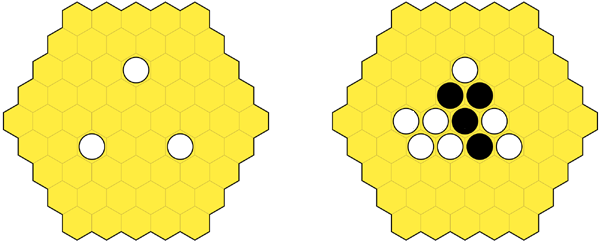
\includegraphics[width=0.95\textwidth]{Abbildungen/yav_triangle.png}
\caption[The triangle starting pattern, Source:\cite{yvalathHP}]{The triangle starting pattern}
\label{fig:yav_triangle}
\end{figure}

In Yavalath a Triangle is always a good pattern, for example the small triangle (as seen in illustration \ref{fig:yav_smallTriangle}). The Reason that the small triangle is such a strong pattern is because it can foram a huge number of winning chances. 


\begin{figure}[ht]
\centering
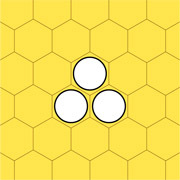
\includegraphics[width=0.45\textwidth]{Abbildungen/yav_smallTriangle.png}
\caption[A small triangle pattern, Source:\cite{yvalathBGG}]{A small triangle pattern}
\label{fig:yav_smallTriangle}
\end{figure}

To show that the small triangle is a good pattern two winning patterns are shown in illustration \ref{fig:yav_smallTriangleWin1} and in illustration \ref{fig:yav_smallTriangleWin2}. Both force the black player to loose by a force move. Also its possible to turn a pattern by 120� Degree, with that in mind there are at least six possible winning situations. If a opponent player try to form a triangle its recommendet to stop him as soon es possible.\cite{yvalathBGG}



\begin{figure}[ht]
\centering
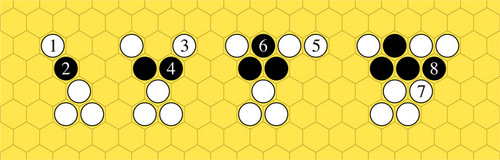
\includegraphics[width=0.95\textwidth]{Abbildungen/yav_smallTriangleWin1.png}
\caption[A small triangle winning pattern, Source:\cite{yvalathBGG}]{A small triangle winning pattern}
\label{fig:yav_smallTriangleWin1}
\end{figure}

\begin{figure}[ht]
\centering
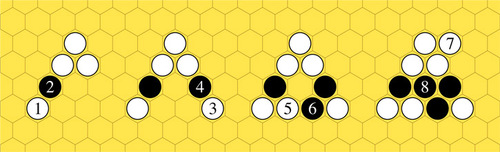
\includegraphics[width=0.95\textwidth]{Abbildungen/yav_smallTriangleWin2.png}
\caption[A second small triangle winning pattern, Source:\cite{yvalathBGG}]{A second small triangle winning pattern}
\label{fig:yav_smallTriangleWin2}
\end{figure}


\chapter{Artificial Intelligences}
\label{sec:artificIntelligences}
The following chapter describes the two approaches of Artificial Intelligences, which were implemented to this Game. The two Artificial Intelligences are able 
to play against a human player and even to win against him. On the one hand there is the so called UTCAI, which can has three different
levels of difficulty. And the other hand there is the simple approach of a random AI. Both approaches are explained in a more detailed view in the next two
sections. 



\section{Random-AI}
The random AI is one of the two implemented Artificial-Intelligences, as already mentioned in the description of this chapter. 
Actually the random AI is defintely the more easier opponent for a human player and also for the other other kind of AI, the UCT AI. 
Additionally to this fact, the random AI is also the more easier approach to implement. Rather the random AI can be described within to sentences : 
Set your tokens randomly, but before you do that, check if you could  win with your next turn or if you must prevent, that one of your opponents could win. 
In a more detailed view this means, the random AI sets its token completely randomly to the playground. This happens with the assistance of a special algorithm, 
which receives the system time. Based on this system time the algorithm can determine a special courton on the playground. If this courton is not used by 
another player, the random AI will set its token there. It doesn't matter if this turn was smart or if it could yield an advantage. But before the random AI 
sets its token, it checks whether a opponent could win on the next turn. This happens based on a predefined rule set, as already mentioned in the chapters above. 
Additionally to that the random AI checks also if it could excel an opponent on the next turn. And all good things are three, so the random AI checks in a third 
step if it could win itself, when it sets the token on a certain courton. All in all the random AI is not very smart, because neither it can deal with specific 
game events nor learning from faults, which were made by the random AI in a game before. It actually sets its token so long as the AI itself could win randomly. 
And this probability is not very high. 


\section{UCT-AI}
\label{sec:chapter4}
The following chapter describes the fundamentals of the UCT (Upper Confidence
Bounds applied to Trees) algorithm. It was implemented in order to provide the
Yavalath game with an artificial intelligence (AI) to play against. The main
task of a game playing AI is to choose its next move with the information about
the state of the game. The motivation and reasons behind choosing the UCT
algorithm are briefly pointed out. Afterwards it is explained how this
algorithms works and how it is integrated into Yavalath.

\subsection{Why UCT?}
The UCT algorithm was developed for decision making problems especially in terms
of game playing. It has its strengths in games where:
\begin{itemize}
	\item the state of a game is hard to evaluatate and
	\item the game has a high branching factor.\footnote{cf. \cite{wiki:mcts}}
\end{itemize}

In Yavalath, these two attributes can be found. Firstly, Yavalath has no
developed theory, mainly because it is relatively unknown, and therefore there
does not exist an evaluation function which could rate the current state of the
game. If it was possible to assign a score depending on how good a player's
tokens are placed on the board, it would be possible to deploy algorithms (such
as Alpha-beta pruning and Minimax), which can leverage this information in order
to find a good or even the best possible next move.\\

Secondly, Yavalath also has a high branching factor. Looking only at the first
10 moves (5 from each player when 2 are playing), there already are
\(\frac{61!}{51!}=3,27*10^17\) different move combinations. Good game playing
AIs cannot only look at the next move, but rather need to look ahead a couple of
moves. Otherwise, they could not detect potential threats or opportunities which
might lie ahead a few moves. In order to investigate all these branches, the AI
needs to be capable of handling the huge number of combinational moves.\\

The UCT algorithm is able to handle both these attributes of Yavalath and
therefore is a reasonable choice for a AI algorithm. This is further justified
by the fact that the creator of Yavalath himself implemented this algorithm as
AI in his Yavalath application. \footnote{\cite{yvalath}}\\

\subsection{How the UCT algorithm works}

The UCT algorithm is based on the Monte Carlo Tree Search (MCTS). The MCTS is a
best-first search algorithm where the results from previous iterations guide the
algorithm to the best path through the tree. It consists of 4 steps which are
run in a loop. The 4 steps\footnote{cf. \cite{mcts}, cf. \cite{wiki:mcts}} are:
\begin{itemize}
	\item \textit{Selection:} Starting at root node R, successively select optimal child nodes until a leaf node L is reached.
	\item \textit{Expansion:}  If L is a not a terminal node, which ends the game, then create one or more child nodes and select one C.
	\item \textit{Simulation:}  Run a simulated playout (usually a random playout) from C until a result is achieved.
	\item \textit{Backpropagation:}  Update the current move sequence from C to R with the simulation result.
\end{itemize}

\begin{figure}[ht]
\centering
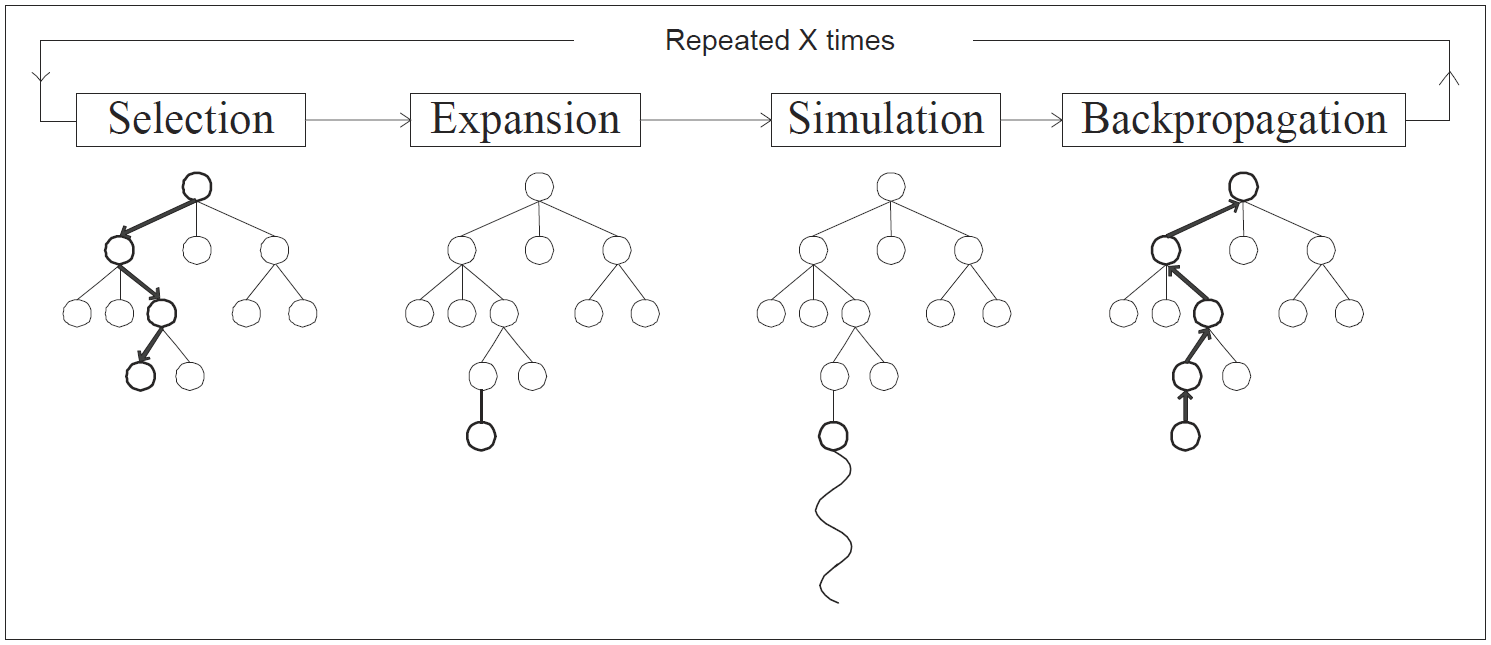
\includegraphics[width=0.95\textwidth]{Abbildungen/MonteCarloTreeSearch.png}
\caption[Monte Carlo Tree Search, Source:\cite{paper:mcts}]{Monte Carlo Tree Search}
\label{fig:yav_winChance}
\end{figure}

In the regard of Yavalath, the root of the tree would represent the current
state of the game. From there the first layer holds all possible next moves the
AI can make. The goal of the AI is now to find the best promising move in that
first layer. Going down one layer, the second layer would represent all possible
counter moves of the following player. In each layer the algorithm tries to find
the best move and expands successive moves to see how the game would evolve when
picking a particular move in the first place. That said, the algorithm also
takes into consideration what the best move for the AI's opponent is. For example,
even though a move seems to be promising in the first layer, the opponent might
be able to counter this move with a very strong response move and thus leading
to a worse situation than initially thought. Therefore, it is important to
further investigate potentially good moves by going down more and more layers,
i.e. rounds of the game. The simulation phase is used to determine the
performance of the moves. Usually, random playouts are used to quickly see how a
game of chosen moves turns out in the end. It might seem that a random playout
cannot be representative, but with more and more playouts the accuracy of the
expected win chance increases due to the law of large numbers.
The result of a random playout is backpropagated to all involved moves till the
root node.\\

It is still unclear how the algorithm chooses a node, and path
respectively, in the selection phase. This is probably the most important part
of the algorithm because it determines the best-first search strategy. The
algorithm needs to find a good balance between exploitation and exploration.
Expoitation is defined as investigating deep variants of the best move sequences
whereas exploration means trying out moves which have not been simulated many
times. The former is important because the AI needs to be confident that the
choice of a move is good even in the further playout and the latter has to be
carried out so that the AI does not miss out on good moves which might just have
unluckily performed bad in a few playouts.\\

To balance out exploitation and exploration the UCB1 (Upper Confidence Bound 1)
policy is used which was first introduced by Peter Auer.\footnote{\cite{paper:ucb1}}
Before using UCB1 in order to decide which node to select from a set of nodes,
every node has to be played out at least once. Afterwards the \(i\)th node is
chosen which maximizes the equation \ref{eq:UCB1}.

\begin{equation}
\label{eq:UCB1}
\bar{x}_{i} + C * \sqrt{\frac{\ln n}{n_{i}}}
\end{equation}

\(x_{i}\) is the performance measure from node \(i\). The performance measure
must lie in the interval [0;1]. For games it usually is the win chance
\(\frac{w_{i}}{n_{i}}\) where \(w_{i}\) is the number of wins from random
playouts of node \(i\) and \(n_{i}\) is the number of times node \(i\) has
already been played. \(n\) is the overall number of playouts and \(C\) is a
constant which has to be adjusted empirically for a given problem. \footnote{cf. \cite{thesis:uct}}\\

In the UCB1 policy, the first part of the equation \(x_{i}\) stands for the
exploitation part. The higher the win chance of a move, the higher the value of
the equation. The rest of the equation stands for the exploration part. Assuming
a node is visited once and not any more for a couple of times, i.e. \(n_{i}\) is
fixed, then only \(n\) increases which makes the overall second part of the
equation grow. On the contrary, for a node which is often visited \(n_{i}\) is
increased simultaneously. As a result, the second part of the equation decreases
because the linear function in the denominator rises faster than the natural
logarithm in the numerator. This means that nodes with a bad win chance and few
plays will eventually be explored too. To what degree and how often they are
explored determines the constant \(C\). The higher the value the more
exploration is done and the lower the value the more exploitation is done.
Auer suggested to set the constant \(C\) to
\(\sqrt{2}\).\footnote{\cite{paper:ucb1}} Therefore, this can be used as a
reasonable starting value.\\

From the UCB1 policy it can be derived that each node needs to to hold two
pieces of information: the number of wins and the number of visits.
Both the MCTS and the UCB1 policy form the UCT algorithm. This explains where
the name Upper Confidence Bounds applied to Trees comes from. The UCT algorithm
could be run quite long on highly branching trees. Fortunately, it can be
stopped at any time. Of course, the longer the algorithm runs the more
statistically significant the result will be, but often a fixed number of
iterations (depending on the problem) are sufficient to get a good result.
The best move will finally be chosen by looking at the information of all nodes
in the first layer. It is best to choose the node which was visited the most.
Even though it is possible to choose the node with the highest win chance, this
might result in a bad move. Through exploration a node can temporarily have a
higher win chance, but as it is probably not exploited very much, it is unclear
if it really is a good move. A high win chance will subsequently result in
higher exploitation and a higher number of visits. Therefore, the number of
visits should be used to make the decision on the best move.


\chapter{Technical Implementation}
\label{sec:technImplementation}
The game was implemented in Java, a platform-independent programming language.
It offers many extensions to develop such a complex game. The aspect that Java
is a object oriented programming language provides many advantages to model
useful classes, which can demonstrate the structure of such a game. Java is also
fast enough to calculate all dependecies and to return the user a
response on their interaction with the game in a suitable time. But therefore
isn't a high-end computer needed. In this context no frameworks were used. The
graphical user interface was realized with the assistance of the GUI-Library
SWING for Java, which is based on the Abstract-Window-Toolkit (AWT).  
\section{implemented Features}
The following section describes the features, which were implemented. \\
After the game was started, the main menu will be opened. The user can start a new game, make settings and exit the game in this menu. Within the settings menu the user is able to define how many player are part of the game (from one to three) and which sort of player each defined player is (human player, random AI or UCT AI). When a player is a UCT AI an additional option is available, namely, which level of difficulty the UCT AI has.
\newpage

\begin{figure}[ht]
\centering
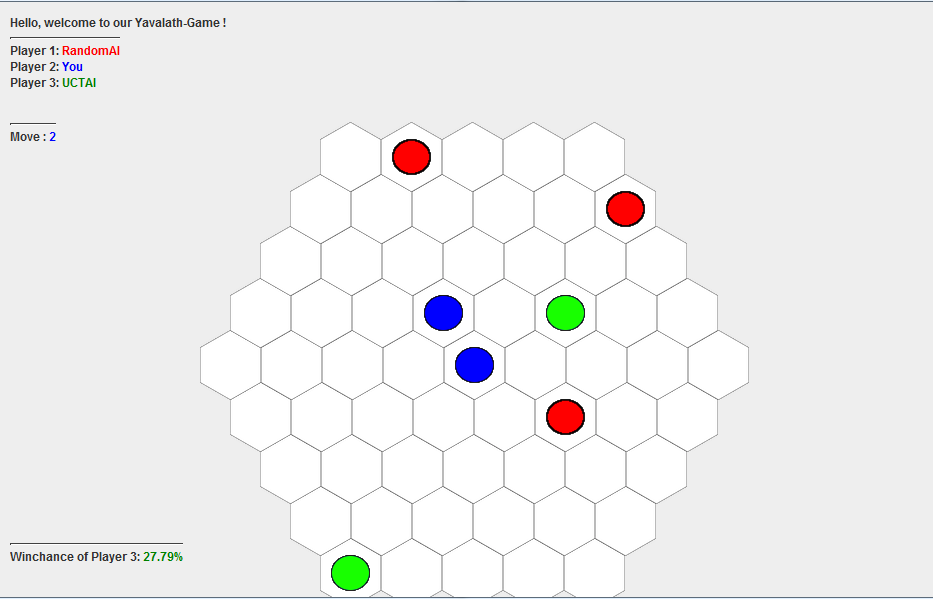
\includegraphics[width=0.95\textwidth]{Abbildungen/exampleOfPlayGround.png}
\caption[Playground of Yavalath implementation]{Playground of Yavalath implementation}
\label{fig:playgroundOfYav}
\end{figure} 

\noindent Figure \ref{fig:playgroundOfYav} shows an example of a typical playground of the Yavalath implementation. 
The upper left corner shows some general game information. Which player has which color and what kind of type the different 
players are. Beneath this information the field 'Move' shows, which players move it is, with the specific color. The field in the 
lower left corner shows the calculated winchance of the UTC AI, presented in percent. If there are multiple UCT AI in the game, the 
certain UCT AI can be indicated by the reference to the color.  \\
The main part of the window is used for the real playground. When it is a human players turn, the player is able to click on the court, 
where he wants to set his 
token. 

\section{Implementation of the UCT-AI}
The implementation of the UCT-AI is primarily based on the theoretical
foundation of the Monte Carlo Tree Search and the UCB1 policy explained in the
previous chapter. This section deals with implementational details such as how
the algorithm was tweaked and how the implementation differs from the theory. 
Sensei's Library features pseudo code for the UCT algorithm which was used as a
basis. \footnote{\cite{sl}}\\

The selection phase of the MCTS uses the UCB1 policy as described before. The
main adjustment done in this part is the choice of the constant \(C\) in the
UCB1 policy from equation \ref{eq:UCB1}. In Sensei's Library, it is suggested to
use a value of \(\frac{1}{sqrt{5}}\).\footnote{\cite{sl}} As this is a smaller
number than \(sqrt{2}\) suggested by Auer, it results in a more exploitational
tree search. Therefore, good moves are investigated more than exploring the
total width of the tree. It turns out that this works very well with Yavalath.\\

The expansion phase is slightly modified. Firstly, when expanding the tree by a
new layer, all children nodes of the currently expanded node are added to the
tree. From the new nodes, a random node is selected. If the path to the newly
added layer is chosen again, each of the nodes is visited at least once before a
definite selection by the UCB1 policy is made. The Monte Carlo Tree Search
suggests to expand the tree as soon as a leaf node is reached. This was modified
by the fact that each node needs to be visited at least 10 times before it is
expanded with its children. This means that the simulation phase would start
right after the selection phase if a leaf node has less than 10 visits. The
reason behind this is to reduce to size of the tree stored in memory and
therefore make the algorithm less prone to run out of memory. The number 10 was
again suggested by the Sensei's Library and works very well in this regard, too.\\

The simulation phase is done with the help of the Random-AI described earlier.
Depending on the number of players, the same number of Random-AI's finish the
game. This phase is the main reason behind some AI logic implemented in the
Random-AI. If the Random-AI would choose its moves completely randomized, it
would also reduce the effectiveness and strength of the UCT-AI. The reason
behind this is that games at the later stage tend to have lots of fields on the
board where a player can lose by placing a third token in a row. The problem
here is that a human player would most likely never do such a move if it is not
forced. Therefore, many simulated games would result in not representative
outcomes, even though it is way more interesting how the game turns out if these
moves are avoided. The same holds for following suit of a forced move or taking
a winning move which is also done by the Random-AI. Having this added logical
improvements in the Random-AI, the simulations done in the UCT algorithm become
much more valuable and representative so that the overall AI increases in
strength.\\

For the backpropagation phase, there is nothing to adjust or modify. It is only
important to keep in mind that for each player the outcome of the simulation is
different (expect for a draw). When having two players, the result of the
simulation has to be alternated on each layer / node when doing the
backpropagation. Accordingly, the result has to be matched with the player of
the current node when dealing with three players.\\

Finally, there are two different ways to execute the UCT algorithm. First, one
can set a fixed time and let the algorithm do as many iterations of the 4 steps
as possible. Second, one can set a fixed number of iterations and have the
algorithm run a somewhat undefined time depending on the power of the CPU on
which it runs. It was decided to implement the second option, because this
enables to define different difficulties (i.e. strengths) of the UCT-AI.
The more iterations there are, the more exploitation as well as exploration the
UCT-AI could do and thus resulting in a better choice of move. Less iterations
mean a weaker AI whereas more iterations make a string AI. Option one with fixed
time does not guarantee the same nummber of iterations on different CPUs and
therefore, the AI would not perform consistently on every PC. In addition, there
should not be a huge difference in execution time, provided that the PC's CPU is
not too outdated. \\

Having experimented and played against the UCT-AI the following number of
iteration were chosen for the corresponding difficulties:
\begin{itemize}
	\item \textit{Easy:} 10000 simulations
	\item \textit{Medium:}  20000 simulations
	\item \textit{Hard:}  50000 simulations
\end{itemize}


% #TODO: Tech the Dokument



\end{document}
